\documentclass{beamer}
\mode<presentation>
\usepackage{amsmath}
\usepackage{amssymb}
%\usepackage{advdate}
\usepackage{adjustbox}
\usepackage{subcaption}
\usepackage{enumitem}
\usepackage{multicol}
\usepackage{mathtools}
\usepackage{listings}
\usepackage{url}
\def\UrlBreaks{\do\/\do-}
\usetheme{Boadilla}
\usecolortheme{lily}
\setbeamertemplate{footline}
{
  \leavevmode%
  \hbox{%
  \begin{beamercolorbox}[wd=\paperwidth,ht=2.25ex,dp=1ex,right]{author in head/foot}%
    \insertframenumber{} / \inserttotalframenumber\hspace*{2ex} 
  \end{beamercolorbox}}%
  \vskip0pt%
}
\setbeamertemplate{navigation symbols}{}

\providecommand{\nCr}[2]{\,^{#1}C_{#2}} % nCr
\providecommand{\nPr}[2]{\,^{#1}P_{#2}} % nPr
\providecommand{\mbf}{\mathbf}
\providecommand{\pr}[1]{\ensuremath{\Pr\left(#1\right)}}
\providecommand{\qfunc}[1]{\ensuremath{Q\left(#1\right)}}
\providecommand{\sbrak}[1]{\ensuremath{{}\left[#1\right]}}
\providecommand{\lsbrak}[1]{\ensuremath{{}\left[#1\right.}}
\providecommand{\rsbrak}[1]{\ensuremath{{}\left.#1\right]}}
\providecommand{\brak}[1]{\ensuremath{\left(#1\right)}}
\providecommand{\lbrak}[1]{\ensuremath{\left(#1\right.}}
\providecommand{\rbrak}[1]{\ensuremath{\left.#1\right)}}
\providecommand{\cbrak}[1]{\ensuremath{\left\{#1\right\}}}
\providecommand{\lcbrak}[1]{\ensuremath{\left\{#1\right.}}
\providecommand{\rcbrak}[1]{\ensuremath{\left.#1\right\}}}
\theoremstyle{remark}
\newtheorem{rem}{Remark}
\newcommand{\sgn}{\mathop{\mathrm{sgn}}}
\providecommand{\abs}[1]{\left\vert#1\right\vert}
\providecommand{\res}[1]{\Res\displaylimits_{#1}} 
\providecommand{\norm}[1]{\lVert#1\rVert}
\providecommand{\mtx}[1]{\mathbf{#1}}
\providecommand{\mean}[1]{E\left[ #1 \right]}
\providecommand{\fourier}{\overset{\mathcal{F}}{ \rightleftharpoons}}
%\providecommand{\hilbert}{\overset{\mathcal{H}}{ \rightleftharpoons}}
\providecommand{\system}{\overset{\mathcal{H}}{ \longleftrightarrow}}
	%\newcommand{\solution}[2]{\textbf{Solution:}{#1}}
%\newcommand{\solution}{\noindent \textbf{Solution: }}
\providecommand{\dec}[2]{\ensuremath{\overset{#1}{\underset{#2}{\gtrless}}}}
\newcommand{\myvec}[1]{\ensuremath{\begin{pmatrix}#1\end{pmatrix}}}
\let\vec\mathbf

\providecommand{\degree}{{^\circ}}

\lstset{
%language=C,
frame=single, 
breaklines=true,
columns=fullflexible
}

\numberwithin{equation}{section}

\newenvironment{amatrix}[2]{%
  \left(\begin{array}{@{}*{#1}{c}|*{#2}{c}@{}}
}{%
  \end{array}\right)
}

\newcommand{\augvec}[3]{\ensuremath{\begin{amatrix}{#1}{#2}#3\end{amatrix}}}

\title{Matrices in Geometry \\ Question 3.3.7}
\author{Shivram S \\ AI24BTECH11031}

\date{\today} 
\begin{document}

\begin{frame}
\titlepage
\end{frame}

\section*{Outline}
\begin{frame}
\tableofcontents
\end{frame}

\section{Problem}

\begin{frame}
\frametitle{Problem Statement}
Write the steps of construction for drawing a $\Delta ABC$ in which $BC = 8$ cm, $\angle B = 45 \degree$ and $\angle C = 30 \degree$.
\end{frame}

\begin{frame}
\frametitle{Information Table}

\begin{table}[h!]
\centering    
\begin{tabular}{| c | c | c |}
   \hline
   \textbf{Variable} & \textbf{Description} & \textbf{Formula} \\ 
   \hline
   $BC$ & Length of the side $BC$ & $BC = 8$ cm \\
   \hline
   $B$ & Measure of the angle at vertex $\vec{B}$ & $B = 45 \degree$ \\
   \hline 
   $C$ & Measure of the angle at vertex $\vec{C}$ & $C = 30 \degree$ \\
   \hline
\end{tabular}
\end{table}

\end{frame}

\section{Solution}
\subsection{Linear Equations}


\begin{frame}
\frametitle{Linear Equations}

Let us assume that $\vec{B} = \myvec{0 \\ 0}$ and $\vec{C} = \myvec{8 \\ 0}$.

We know that
\begin{align}
    \overrightarrow{BA} + \overrightarrow{AC} = \overrightarrow{BC} \implies
    \myvec{c \cos B \\ c \sin B} + \myvec{b \cos C \\ -b \sin C} = \myvec{8 \\ 0} \\
\end{align}
This can be written as a pair of linear equations in $b$ and $c$.
\begin{align} 
    \myvec{\cos C & \cos B \\ -\sin C & \sin B} \myvec{b \\ c} &= \myvec{8 \\ 0} \\
    \myvec{
        \frac{\sqrt{3}}{2} & \frac{1}{\sqrt{2}} \\
        -\frac{1}{2} & \frac{1}{\sqrt{2}}
    } \myvec{b \\ c} &= \myvec{8 \\ 0}
\end{align}
\end{frame}

\subsection{Row Reduction}
\begin{frame}

\frametitle{Row Reduction}

By performing row reduction,

\begin{align}
    \augvec{2}{1}{
        \frac{\sqrt{3}}{2} & \frac{1}{\sqrt{2}} & 8 \\
        -\frac{1}{2} & \frac{1}{\sqrt{2}} & 0
    }
    \xleftrightarrow[]{R_1 \leftarrow R_1-R_2}
    \augvec{2}{1}{
        \frac{\sqrt{3} + 1}{2} & 0 & 8 \\
        -\frac{1}{2} & \frac{1}{\sqrt{2}} & 0
    } \\
    \xleftrightarrow[]{R_1 \leftarrow \frac{2R_1}{\sqrt{3} + 1}}
    \augvec{2}{1}{
        1 & 0 & \frac{16}{\sqrt{3} + 1} \\
        -\frac{1}{2} & \frac{1}{\sqrt{2}} & 0
    } \\
    \xleftrightarrow[]{R_2 \leftarrow 2R_2 + R_1}
    \augvec{2}{1}{
        1 & 0 & \frac{16}{\sqrt{3} + 1} \\
        0 & \sqrt{2} & \frac{16}{\sqrt{3} + 1}
    } \\
    \xleftrightarrow[]{R_2 \leftarrow \frac{R_2}{\sqrt{2}}}
    \augvec{2}{1}{
        1 & 0 & \frac{16}{\sqrt{3} + 1} \\
        0 & 1 & \frac{8\sqrt{2}}{\sqrt{3} + 1}
    }
\end{align}
\end{frame}

\subsection{Solving for A}
\begin{frame}
\frametitle{Solving for A}
Thus,
\begin{align}
    b = \frac{16}{\sqrt{3} + 1}, c = \frac{8\sqrt{2}}{\sqrt{3} + 1} \label{eq:bc}
\end{align}

We can now substitute values from (\ref{eq:bc}) to obtain

\begin{align}
    \vec{A} = \myvec{c\cos B \\ c\sin B} = \myvec{\frac{8}{\sqrt{3} + 1} \\ \frac{8}{\sqrt{3} + 1}}
\end{align}
\end{frame}

\section{Plotting}
\subsection{C Code}
\begin{frame}[allowframebreaks]
\frametitle{C Code}
    The following C program was used to calculate the value of $\vec{A}$:

    \lstset{
        language=C,
        basicstyle=\ttfamily\small,
        keywordstyle=\color{blue},
        stringstyle=\color{purple},
        commentstyle=\color{gray},
        tabsize=4
    }
    \lstinputlisting{codes/generate.c}
\end{frame}

\subsection{Python Code}
\begin{frame}[allowframebreaks]
\frametitle{Python Code}
    The following Python program was used to plot the triangle:

    \lstset{
        language=Python,
        basicstyle=\ttfamily\small,
        keywordstyle=\color{blue},
        stringstyle=\color{purple},
        commentstyle=\color{gray},
        tabsize=4
    }
    \lstinputlisting{codes/plot.py}
\end{frame}

\subsection{Plot}
\begin{frame}    
\frametitle{Plot}
\begin{figure}[h!]
    \centering
    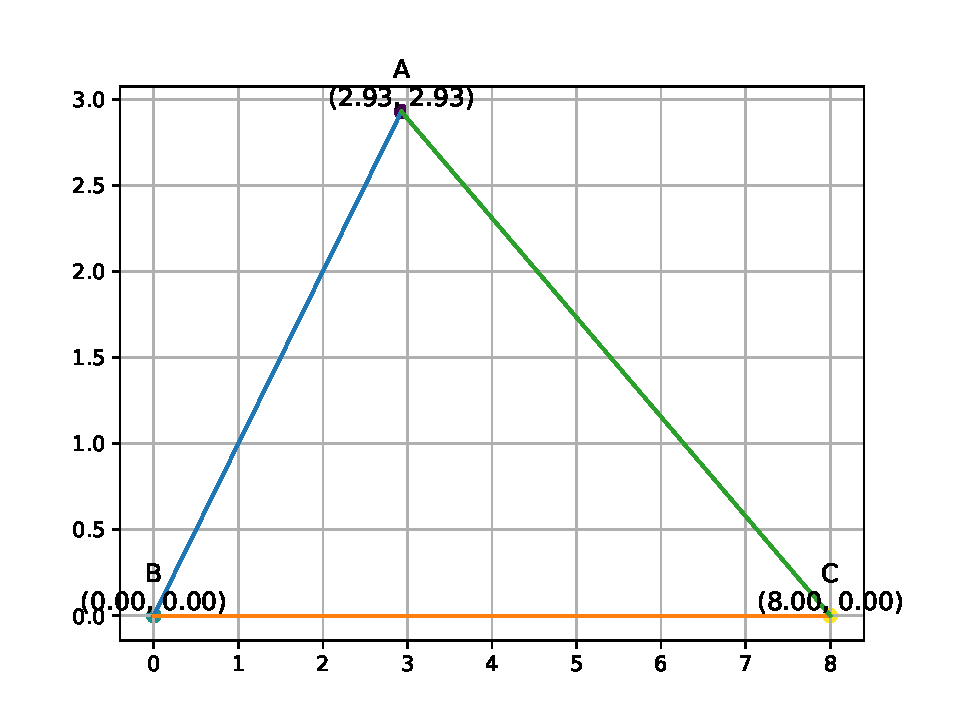
\includegraphics[width=0.7\linewidth]{figs/fig.pdf}
    \caption{Triangle $ABC$ where $BC=8cm$, $\angle B = 45 \degree$ and $\angle C = 30 \degree$}
\end{figure}

\end{frame}

\end{document}
